\documentclass{article}
\usepackage{tikz}
\usepackage{float}
\usepackage{enumerate}
\usepackage{amsmath}
\usepackage{bm}
\usepackage{indentfirst}
\usepackage{siunitx}
\usepackage[utf8]{inputenc}
\usepackage{graphicx}
\graphicspath{ {Images/} }
\usepackage{float}
\usepackage{mhchem}
\usepackage{chemfig}
\allowdisplaybreaks

\title{ 8.01 Problem Set 10 }
\author{ Robert Durfee - Lecture 7 - Table 9}
\date{ November 14, 2017 }

\begin{document}

\maketitle

\section{ Torque and Angular Momentum for a System }

\subsection*{Part A}

Consider the following diagram which shows one mass of a system of $N$ different
masses each travelling with a different velocity:

\begin{figure}[H]
    \centering
    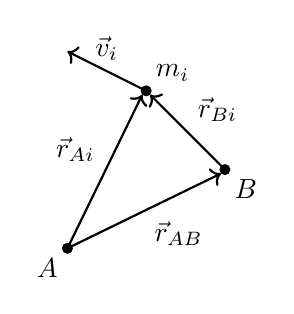
\begin{tikzpicture}
        \fill (0,0) circle (2pt) node[anchor=north east]{$A$};
        \fill (2,1) circle (2pt) node[anchor=north west]{$B$};
        \fill (1,2) circle (2pt) node[anchor=south west]{$m_i$};
        \draw [thick, ->] (0,0) -- (0.95,1.95) node[pos=0.5, anchor=south
        east]{$\vec{r}_{Ai}$};
        \draw [thick, ->] (0,0) -- (1.95,0.95) node[pos=0.5, anchor=north
        west]{$\vec{r}_{AB}$};
        \draw [thick, ->] (2,1) -- (1.05,1.95) node[pos=0.5, anchor=south
        west]{$\vec{r}_{Bi}$};
        \draw [thick, ->] (1,2) -- (0,2.5) node[pos=0.5,
        anchor=south]{$\vec{v}_i$};
    \end{tikzpicture}
\end{figure}

The angular momentum of the system, about axis $A$, can be given by:
$$\vec{L}_A = \sum \limits_{i=1}^{N} \left( \vec{r}_{Ai} \times m_i \vec{v}_i
\right)$$

The angular momentum of the system, about axis $B$, can be given by:
$$\vec{L}_B = \sum \limits_{i=1}^{N} \left( \vec{r}_{Bi} \times m_i \vec{v}_i
\right)$$

Using vector addition, we can define $\vec{r}_{Ai}$ in terms of $\vec{r}_{Bi}$:
$$\vec{r}_{Ai} = \vec{r}_{Bi} + \vec{r}_{AB}$$

This can be used to rewrite the angular momentum of the system on axis $A$:
$$\vec{L}_A = \sum \limits_{i=1}^{N} \left( \left( \vec{r}_{Bi} + \vec{r}_{AB}
\right) \times m_i \vec{v}_i \right)$$

Since $\vec{r}_{AB}$ is a constant, this too can be rewritten:
$$\vec{L}_A = \sum \limits_{i=1}^{N} \left( \vec{r}_{Bi} \times m_i \vec{v}_i
\right) + \sum \limits_{i=1}^{N} \left( \vec{r}_{AB} \times m_i \vec{v}_i
\right)$$

Noticing this includes our definition of linear momentum and $\vec{L}_{B}$, we can
rewrite this as the following:
$$\vec{L}_A = \vec{L}_B + \vec{r}_{AB} \times \vec{p}_{sys}$$

Therefore, whenever the linear momentum of the system is zero, the angular
momentum is the same along any axis. This frame of reference is the center of
mass reference frame because that is where linear momentum is defined to be
zero.

This is helpful in elastic collisions because we can choose any axis about which
to calculate angular momentum and not worry about the differnces between
choices. (As long as the axes are chosen along the center of mass reference
frame, which could be moving if both objects are traveling in the same
direction.)

\subsection*{Part B}

Consider the following diagram which shows one mass of a system of $N$ different
masses each experiencing a different force:

\begin{figure}[H]
    \centering
    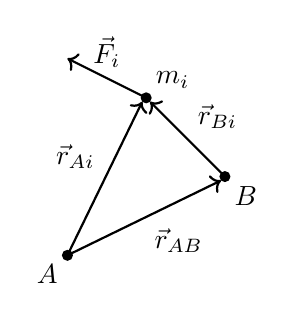
\begin{tikzpicture}
        \fill (0,0) circle (2pt) node[anchor=north east]{$A$};
        \fill (2,1) circle (2pt) node[anchor=north west]{$B$};
        \fill (1,2) circle (2pt) node[anchor=south west]{$m_i$};
        \draw [thick, ->] (0,0) -- (0.95,1.95) node[pos=0.5, anchor=south
        east]{$\vec{r}_{Ai}$};
        \draw [thick, ->] (0,0) -- (1.95,0.95) node[pos=0.5, anchor=north
        west]{$\vec{r}_{AB}$};
        \draw [thick, ->] (2,1) -- (1.05,1.95) node[pos=0.5, anchor=south
        west]{$\vec{r}_{Bi}$};
        \draw [thick, ->] (1,2) -- (0,2.5) node[pos=0.5,
        anchor=south]{$\vec{F}_i$};
    \end{tikzpicture}
\end{figure}

The torque on the system, about axis $A$, can be given by:
$$\vec{\tau}_A = \sum \limits_{i=1}^{N} \left( \vec{r}_{Ai} \times \vec{F}_i
\right)$$

The torque on the system, about axis $B$, can be given by:
$$\vec{\tau}_B = \sum \limits_{i=1}^{N} \left( \vec{r}_{Bi} \times \vec{F}_i
\right)$$

Using vector addition, we can define $\vec{r}_{Ai}$ in terms of $\vec{r}_{Bi}$:
$$\vec{r}_{Ai} = \vec{r}_{Bi} + \vec{r}_{AB}$$

This can be used to rewrite the torque on the system on axis $A$:
$$\vec{\tau}_A = \sum \limits_{i=1}^{N} \left( \left( \vec{r}_{Bi} + \vec{r}_{AB}
\right) \times \vec{F}_i \right)$$

Pulling out constants and the definition of $\vec{\tau}_{B}$:
$$\vec{\tau}_A = \vec{\tau}_B + \vec{r}_{AB} \times \vec{F}_{sys}$$

Therefore, whenever the total force on the system is zero (i.e. the system is
not accelerating and is in equilibrium), the torque is the same on the same
along any axis. 

This is helpful in static equilibrium problems because we can choose any axis
that we would like without worrying about the differences between choices.

\section{Toy Locomotive}

In this problem, it is important to note that the angular momentum is the same
for the system before and after the car accelerates.

Prior to the car's acceleration, both the track and the car are at rest.
Therefore, total momentum is: 
$$\vec{L}_{sys} = 0$$

After the car's acceleration, the momentum must remain zero. Therefore, we can
write an expression for the angular momentum after the car reaches it's final
velocity as:
$$\vec{0} = -\vec{L}_{lf} + \vec{L}_{tf}$$

Defining the angular momentums in terms of our given variables results in:
$$R \times m_l \vec{v}_{lf} = m_t R \vec{v}_{tf}$$

Given that the car moves tangentially along the track and that the angular
momentums are both in $\hat{k}$ direction:
$$m_l v_{lf} = m_t v_{tf}$$

However, since we are not given $v_{tf}$, rather, we are given $v$, using the
definition of relative velocity:
$$v_{lf} = v - v_{tf}$$

Now we can write our equation in terms of $v$:
\begin{align*}
    m_l v_{lf} &= m_t \left( v - v_{lf} \right) \\
    m_l v_{lf} + m_t v_{lf} &= m_t v \\
    v_{lf} &= \frac{m_t}{m_t + m_l} v
\end{align*}

\section{A Spaceship and a Planet}

In this problem, it is important to note that the angular momentum and energy or
the system is constant for spaceship 2.

First, we can solve for the speed of the first spaceship by setting centripetal
force equal to the gravitational force:
$$\frac{m_1 v_1^2}{R} = \frac{G m_p m_1}{R^2}$$

Solving for $v_1$ results in:
$$v_1 = \sqrt{ \frac{G m_p}{R} }$$

Now, setting the initial and final angular momentum of spaceship 2 equal:
\begin{align*}
    3 R m_2 v_2 &= R m_2 v_p \\
    3 v_2 &= v_p
\end{align*}

Now, setting the initial and final energy of spaceship 2 equal:
\begin{align*}
    \frac{1}{2} m_2 v_2^2 - \frac{G m_p m_2}{3 R} &= \frac{1}{2} m_2 v_p^2 -
    \frac{G m_p m_2}{R} \\
    v_2^2 &= v_p^2 - \frac{4 G m_p}{3 R}
\end{align*}

Substituting this into the angular momentum equation:
\begin{align*}
    3 \left( v_p^2 - \frac{4 G m_p}{3 R} \right) &= v_p^2 \\
    v_p = \sqrt{ \frac{3 G m_p}{2R} }
\end{align*}

Solving for the difference between $v_1$ and $v_p$:
$$\Delta v = \sqrt{ \frac{G m_p}{R} } - \sqrt{ \frac{3 G m_p}{2R} }$$

Since $v_p$ is larger than $v_1$, the second spaceship must slow down to dock
alongside the first spaceship.

\section{Satellite Maneuver}

In this problem, the angular momentum and energy are constant.

Setting the initial and final angular momentum of the package equal:
\begin{align*}
    \vec{r}_i \times m \vec{v}_i &= \vec{r}_f \times m \vec{v}_f \\
    r_i m v_i \sin(\theta_i) &= r_f m v_f \sin(\theta_f) \\
    r_i v_i \sin(\theta_i) &= r_f v_f \sin(\theta_f)
\end{align*}

Setting the initial and final energy of the package equal:
\begin{align*}
    \frac{1}{2} m v_i^2 - \frac{G M_E m}{r_i} &= \frac{1}{2} m v_f^2 - \frac{G
    M_E m}{r_f} \\
    v_i^2 &= v_f^2 + 2 G M_E \left( \frac{1}{r_i} - \frac{1}{r_f} \right)
\end{align*}

Substituting into the angular momentum equation:
\begin{align*}
    r_f^2 v_f^2 \sin^2(\theta_f) &= r_i^2 \sin^2(\theta_i) \left( v_f^2 + 2 G 
    M_E \left( \frac{1}{r_i} - \frac{1}{r_f} \right) \right) \\
    v_f &= \sqrt{ \frac{ 2 G M_E r_i^2 \sin^2(\theta_i) }{ r_f^2
    \sin^2(\theta_f) - r_i^2 \sin^2(\theta_i) } \left( \frac{1}{r_i} - 
    \frac{1}{r_f} \right) }
\end{align*}

\section{A Rigid Rod}

\subsection*{Part A}

\begin{itemize}
    \item \textbf{Energy} - In this case, the three objects collide in a way
        such that they stick together. This is an inelastic collision. As a
        result, the energy is not conserved.

    \item \textbf{Linear Momentum} - The effect after the collision not only
        depends on the initial velocities of the two objects about the hit the
        pivoted rod, but also the distance from the axis where they will hit. If
        one object is further away, it will produce a greater torque, even if
        the velocity is the same as the other. As a result, linear momentum is
        not conserved.

    \item \textbf{Angular Momentum} - Since the angular momentum take into
        effect the position where the objects will hit the rod, angular momentum
        will be conserved.
\end{itemize}

\subsection*{Part B}

Setting the initial and final angular momentum equal:
\begin{align*}
    \frac{2 d}{3} m v - \frac{d}{3} m v &= \left( m \left( \frac{d}{3} \right)^2
    + m \left( \frac{2 d}{3} \right)^2 + \frac{1}{3} m d^2 \right) \omega \\
    \omega &= \frac{3 v}{8 d}
\end{align*}

\subsection*{Part C}

Solve for the iniial kinetic energy:
$$KE_i = m v^2$$

Solve for the final kinetic energy:
\begin{align*}
    KE_f &= \frac{1}{2} \left( m \left( \frac{d}{3} \right)^2 + m \left( \frac{2 d}{3}
    \right)^2 + \frac{1}{3} m d^2 \right) \omega^2 \\
    KE_f &= \frac{1}{16} m v^2
\end{align*}

Defining the ratio of the change in kinetic energy to the initial kinetic
energy:
\begin{align*}
    \frac{ m v^2/16 - m v^2}{m v^2} = -\frac{15}{16}
\end{align*}

\section{Elastic Collision of Object and Pivoted Ring}

Setting initial and final angular momentum equal:
$$R m v_0 = I \omega - R m v_f$$

Setting initial and final kinetic energy equal:
$$\frac{1}{2} m v_0^2 = \frac{1}{2} I \omega^2 + \frac{1}{2} m v_f^2$$

Solving the angular momentum equation for $\omega$:
$$\omega = \frac{R m (v_0 + v_f)}{I}$$

Substituting $\omega$ into the kinetic energy equation:
\begin{align*}
    m v_0^2 &= I \left( \frac{R m (v_0 + v_f)}{I} \right)^2 + m v_f^2 \\
    m v_0^2 &= \frac{ R^2 m^2 }{I} \left( v_0^2 + 2 v_0 v_f + v_f^2) + m v_f^2
\end{align*}

Rearranging into a quadratic equation:
\begin{align*}
    0 &= -v_0^2 \left( 1 - \frac{R^2 m}{I} \right) + \left( \frac{2 R^2 m
    v_0}{I} \right) v_f + \left( \frac{R^2 m}{I} + 1 \right) v_f^2
\end{align*}

Solving for $I$ using the parallel axis theorem:
\begin{align*}
    I &= I_{cm} + m d^2 \\
    I &= m_R R^2 + m_R R^2 \\
    I &= 2 m_R R^2
\end{align*}

Substituting $I$ into quadratic equation:
$$ 0 = -v_0^2 \left( 1 - \frac{m}{2 m_R} \right) + \left( \frac{m v_0}{m_R}
\right) v_f + \left( \frac{m}{2 m_R} + 1 \right) v_f^2$$

Solving using quadratic formula:
$$ v_f = \frac{ -\frac{m v_0}{m_R} + \sqrt{ \left( \frac{m v_0}{m_R} \right)^2 +
v_0^2 \left( \frac{m}{m_R} + 2 \right) \left( 2 - \frac{m}{m_R}
\right) }}{ \left( \frac{m}{m_R} + 2 \right)}$$

\section{Sand Leaking from a Drum}

First of all, it is important to note that there are no external forces (or
torques) acting on this system. As a result, angular momentum will be conserved.
Additionally, the sand is free to move within the first drum. As a result, as
the sand is flowing from the inner drum to the outer drum, there will be no
effect on the inner drums motion.
$$\omega_A(t) = \omega_{A0}$$

However, after the sand hits the outer drum, it sticks to it. This creates an
inelastic angular collision that will alter the motion of the second drum.
Equating the initial and final momentum of the system (assuming for now all the
sand is transfered):
\begin{align*}
    m_A a^2 \omega_{A0} + m_S a^2 \omega_{A0} &= m_A a^2 \omega_{A0} + (m_B +
    m_S) b^2 \omega_{Bf} \\
    m_S a^2 \omega_{A0} &= (m_B + m_S) b^2 \omega_{Bf}
\end{align*}

Solving for $\omega_{Bf}$:
$$\omega_{Bf} = \frac{m_S a^2 \omega_{A0}}{(m_B + m_S) b^2}$$

Given that we know the rate of transfer of sand, 
$$m_s(t) = \lambda t$$

Substituting this into the conservation of momentum equation:
\begin{align*}
    \omega_{Bf}(t) &= \frac{m_S(t) a^2 \omega_{A0}}{(m_B + m_S(t)) b^2} \\
    \omega_{Bf}(t) &= \frac{\lambda t a^2 \omega_{A0}}{(m_B + \lambda t) b^2}
\end{align*}

\end{document}
